Como se puede obserar en la \textbf{Figura \ref{fig: Arquitectura_Fisica}}, la arquitectura utilizada para el sistema es de tres capas: cliente, servidor, base de datos. Analizando la arquitectura, por el lado de cliente se puede apreciar que sólo se está diseñando para que el sistema sea utilizado a través de PC o Laptop. En cuanto al servidor, se puede destacar que el sistema está montado en un servidor diferente al de la base de dato con el fin de que lo datos no vean comprometidos en caso de que vulneraran el servidor web.

\begin{figure}[htb]
    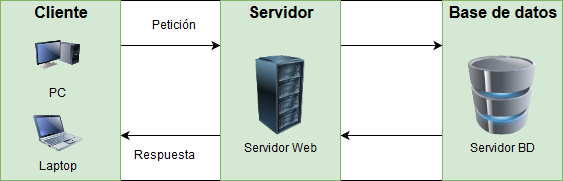
\includegraphics[width=\textwidth]{Imagenes/Arquitectura_Fisica.png}
    \caption{\label{fig: Arquitectura_Fisica}Arquitectura física del sistema.}
\end{figure}